\section{\Large PROBLEM SET 10}

\subsection{Coupling Reaction Wheels with Control Law}

Using the properties of the aforementioned Bradford reaction wheels, a saturation limit was placed on the rate change in angular momentum of each wheel corresponding to the maximum 0.265 Nm that each wheel is capable of outputting. Additionally, a saturation was imposed upon the angular momentum being stored in each wheel. This matches the 45 Nms that each wheel can store. In addition to saturation limits, a first-order linear transfer function was used to emulate the 80ms rise time between the commanded change in wheel momentum and the actual change being experienced by the system.
The feedback control law is used to generated a moment command that is converted into a commanded change in angular momentum, and the physics model described above is used to calculate the actual output torque made available by the actuators. The Simulink model shown in Figure \ref{fig:}. The inputs and outputs of this simulation are seen in Figure \ref{fig:reaction_wheel_outputs}. The control law is shown to maintain error along each axis to an order of magnitude of $10^{-3}$ radians in Figure \ref{fig:alpha_history_with_full_wheel_model}.

\begin{figure}[H]
    \centering
    \captionsetup{ justification = centering }
    \includegraphics{}
    \caption{Simulink Model Used for Reaction Wheel Physics Model}
    \label{fig:enter-label}
\end{figure}

\begin{figure}[H]
    \centering
    \captionsetup{ justification = centering}
    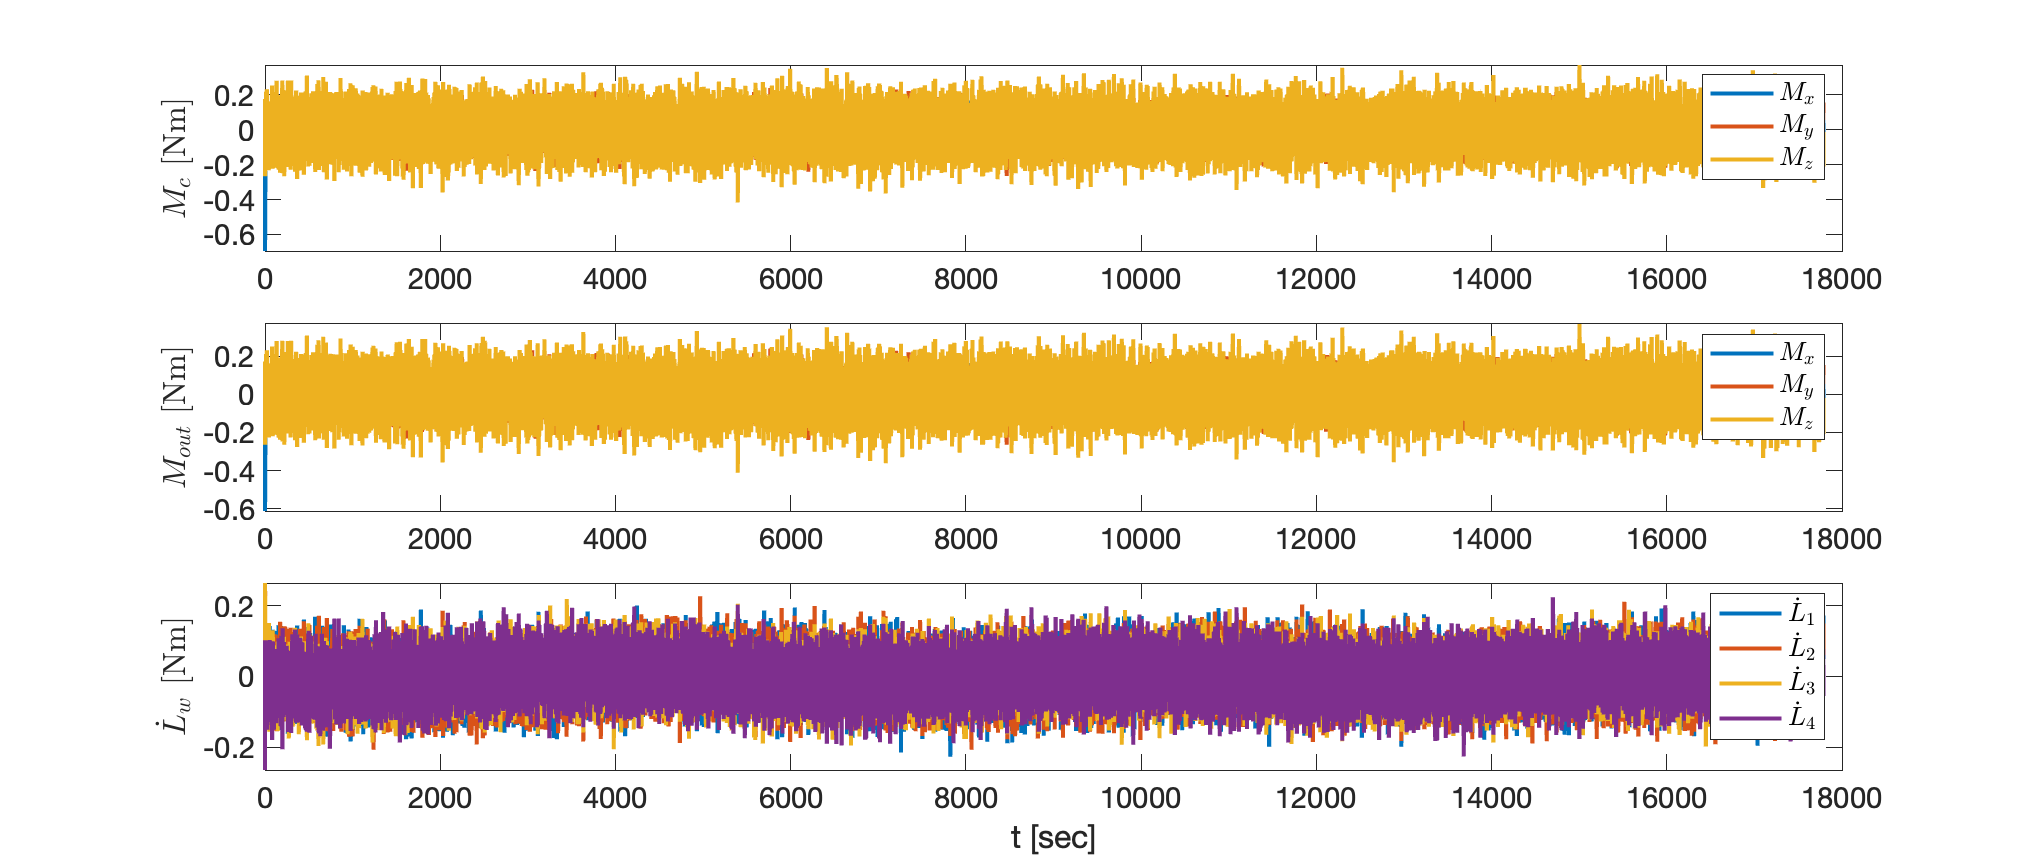
\includegraphics[width=15cm]{Images/PS10/reaction_wheel_model_output.png}
    \caption{Time History of Control Law Input, Actuator Output, and Reaction Wheel Momentum Command}
    \label{fig:reaction_wheel_outputs}
\end{figure}

\begin{figure}[H]
    \centering
    \captionsetup{ justification = centering}
    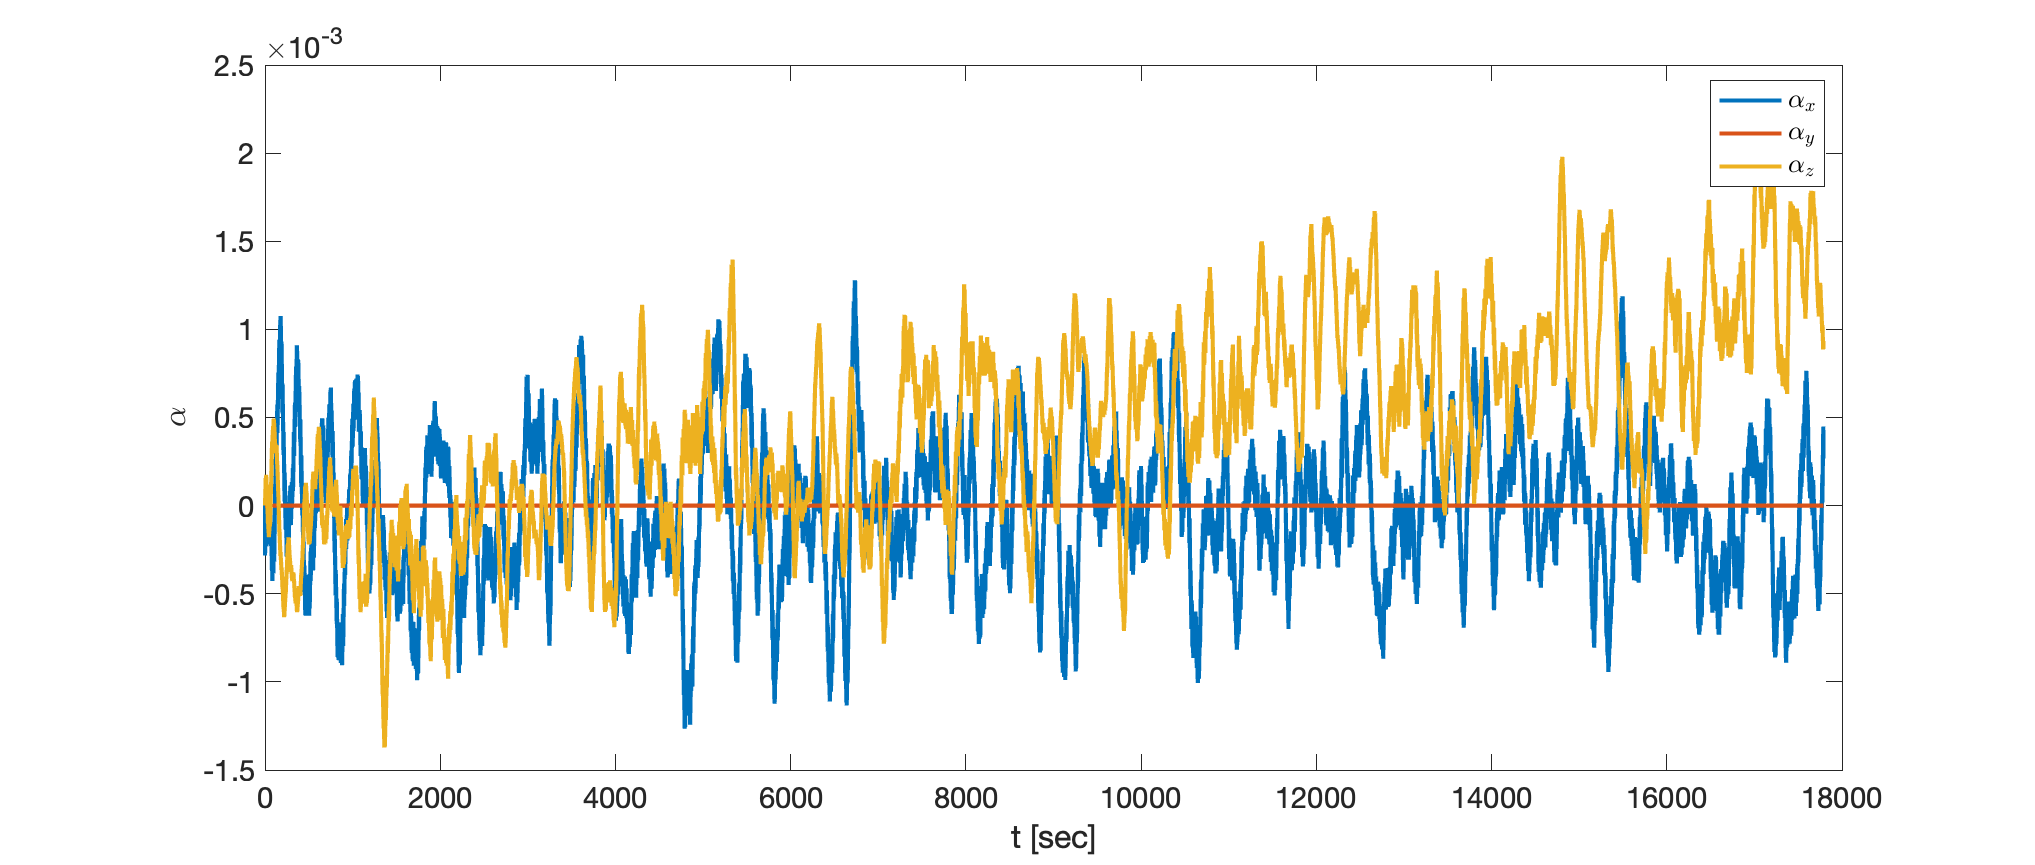
\includegraphics[width=15cm]{Images/PS10/alpha_history_PD_control.png}
    \caption{Time History of Alpha Error}
    \label{fig:alpha_history_with_full_wheel_model}
\end{figure}

\subsection{Basic MEKF Completion and Integration with Feedback Control}

After fixing the measurement model, the MEKF estimated output was fed into the control law. Figures \ref{fig:mekf_attitude_and_error_history} and \ref{fig:mekf_velocity_and_error_history} show that the MEKF output is accurately tracking the ground truth atitiude and velocity.

\begin{figure}[H]
    \centering
    \captionsetup{ justification = centering}
    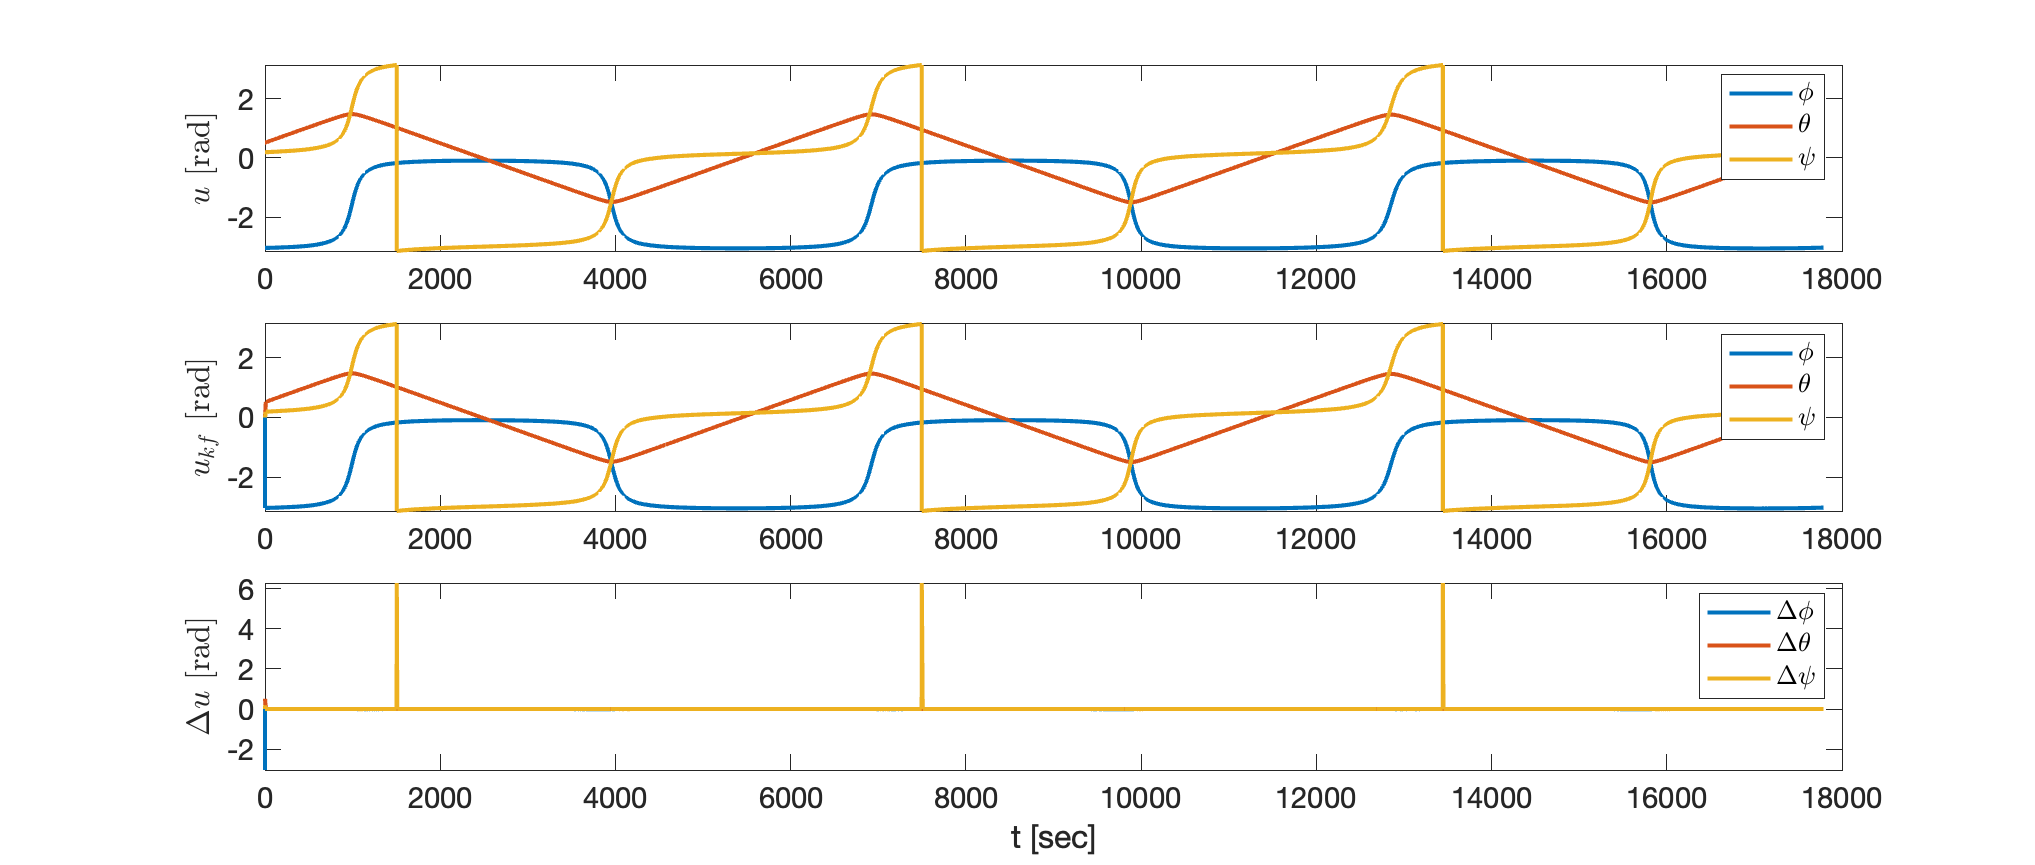
\includegraphics[width=12cm]{Images/PS10/mult_ext_kalman_filter_attitude.png}
    \caption{Time History of Ground Truth Attitude, MEKF Attitude Estimate, and Attitude Determination Error}
    \label{fig:mekf_attitude_and_error_history}
\end{figure}

\begin{figure}[H]
    \centering
    \captionsetup{ justification = centering}
    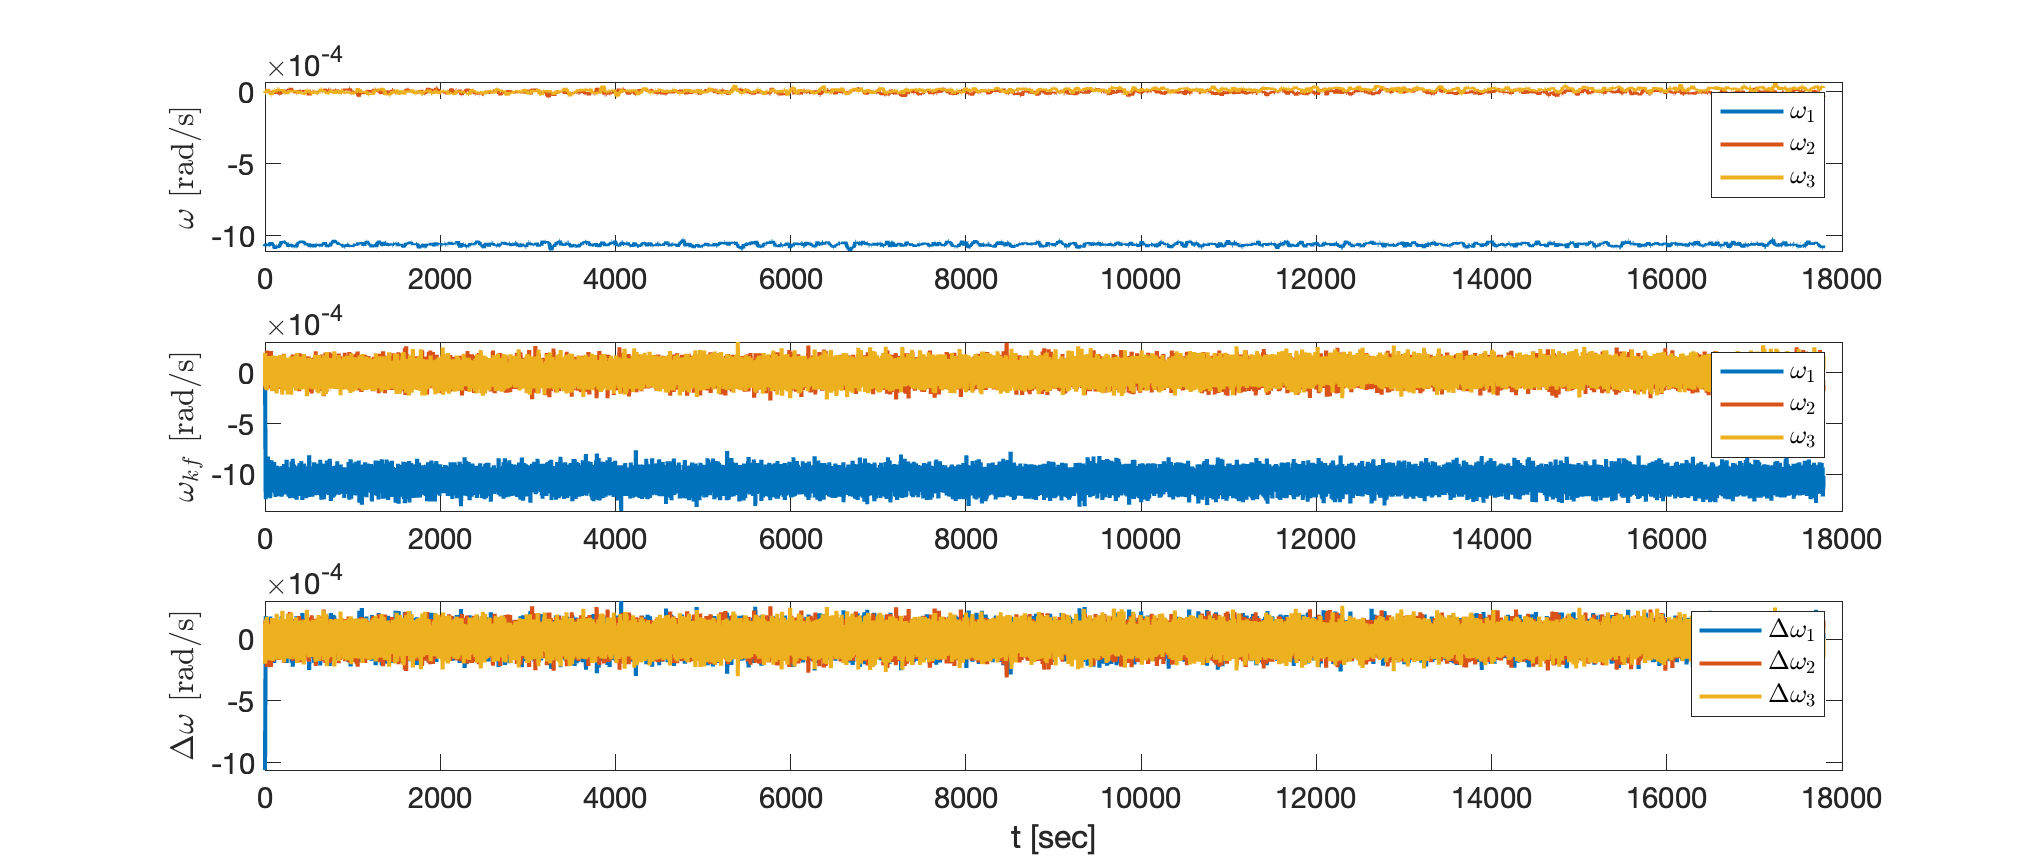
\includegraphics[width=12cm]{Images/PS10/mult_ext_kalman_filter_velocities.png}
    \caption{Time History of Ground Truth Angular Velocity, MEKF Velocity Estimate, and Velocity Estimate Error}
    \label{fig:mekf_velocity_and_error_history}
\end{figure}

Figures \ref{fig:attitude_error_bounds} and \ref{fig:velocity_error_bounds} show the covariance for each estimated parameter centered about the estimated mean. Over this is plotted the ground truth state.

\begin{figure}[H]
    \centering
    \captionsetup{ justification = centering}
    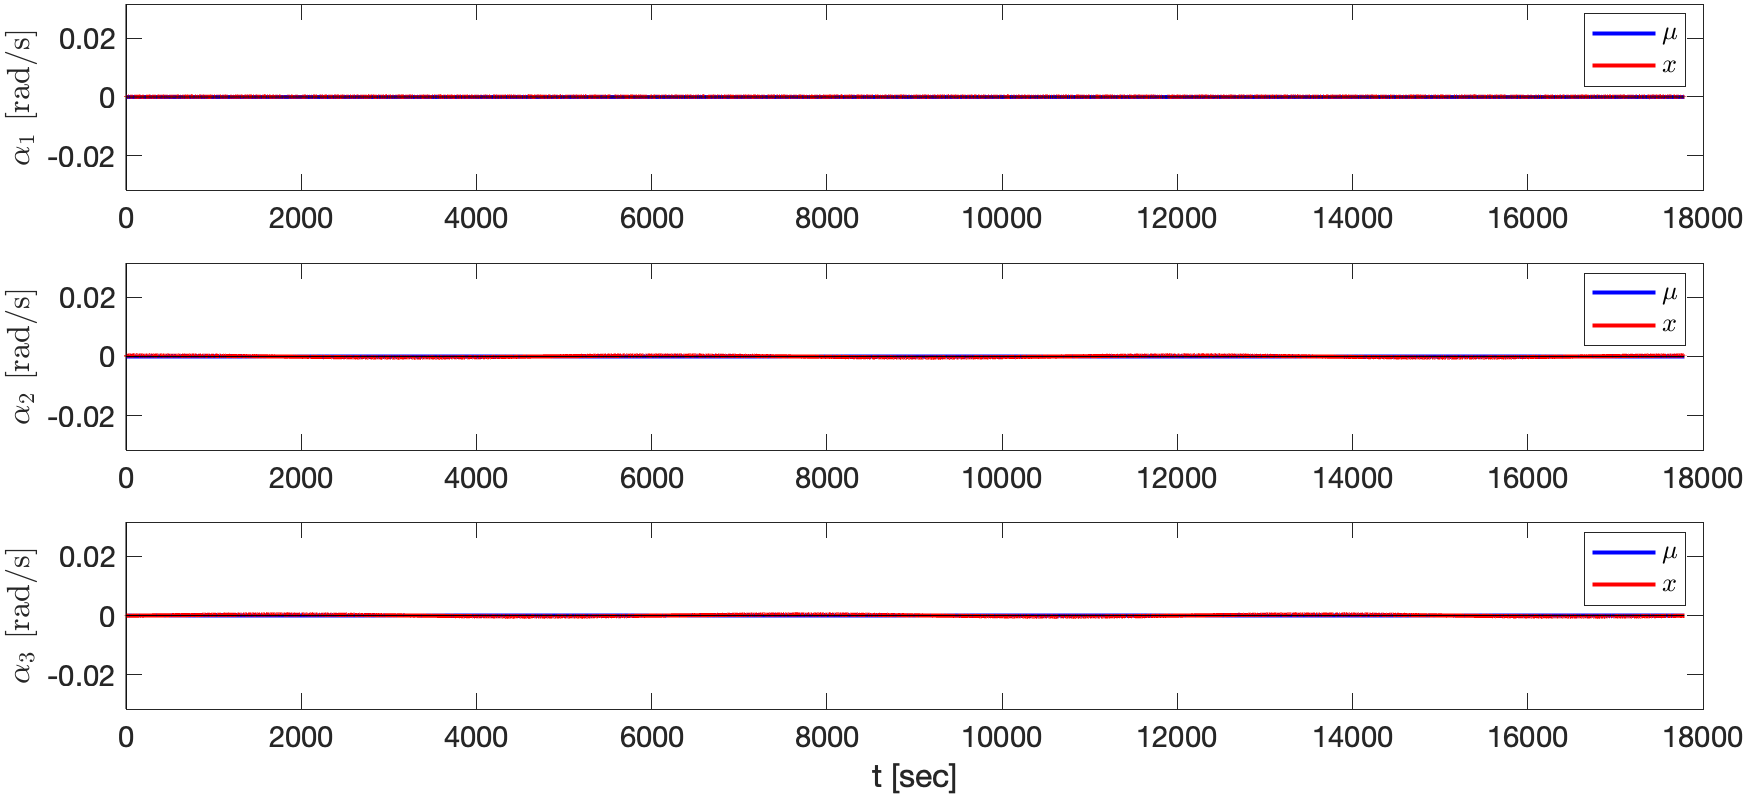
\includegraphics[width=12cm]{Images/PS10/mult_ext_kalman_filter_att_cov_bounds.png}
    \caption{1-$\sigma$ Covariance Bounds on Error State Estimate along with True Error}
    \label{fig:attitude_error_bounds}
\end{figure}

\begin{figure}[H]
    \centering
    \captionsetup{ justification = centering}
    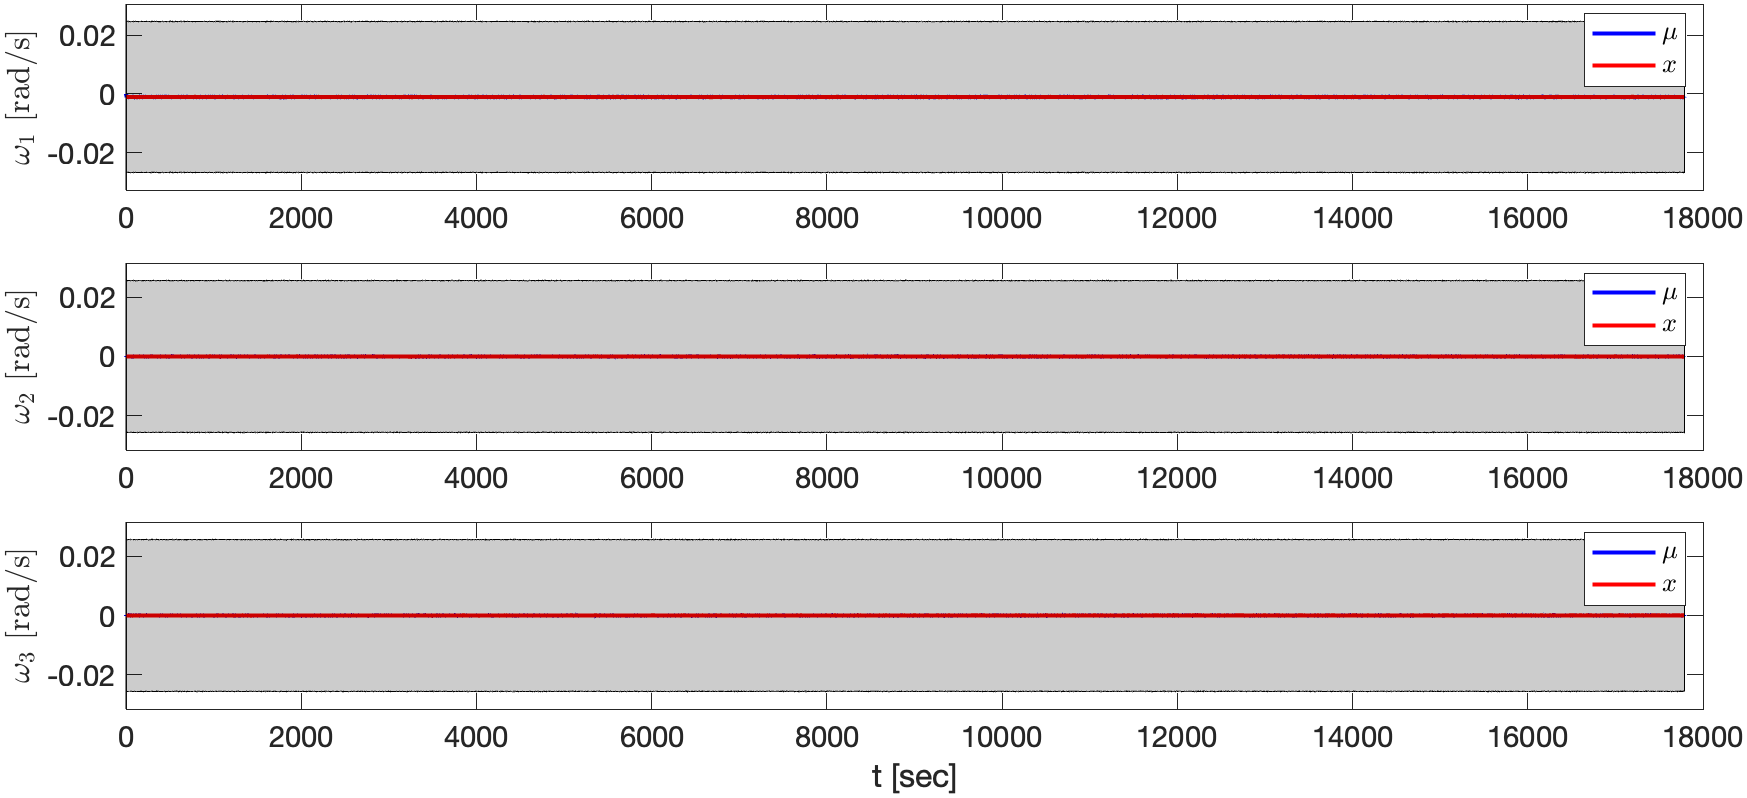
\includegraphics[width=12cm]{Images/PS10/mult_ext_kalman_filter_omega_cov_bounds.png}
    \caption{1-$\sigma$ Covariance Bounds on Velocity Estimate along with True Velocities}
    \label{fig:velocity_error_bounds}
\end{figure}

\begin{figure}[H]
    \centering
    \captionsetup{ justification = centering}
    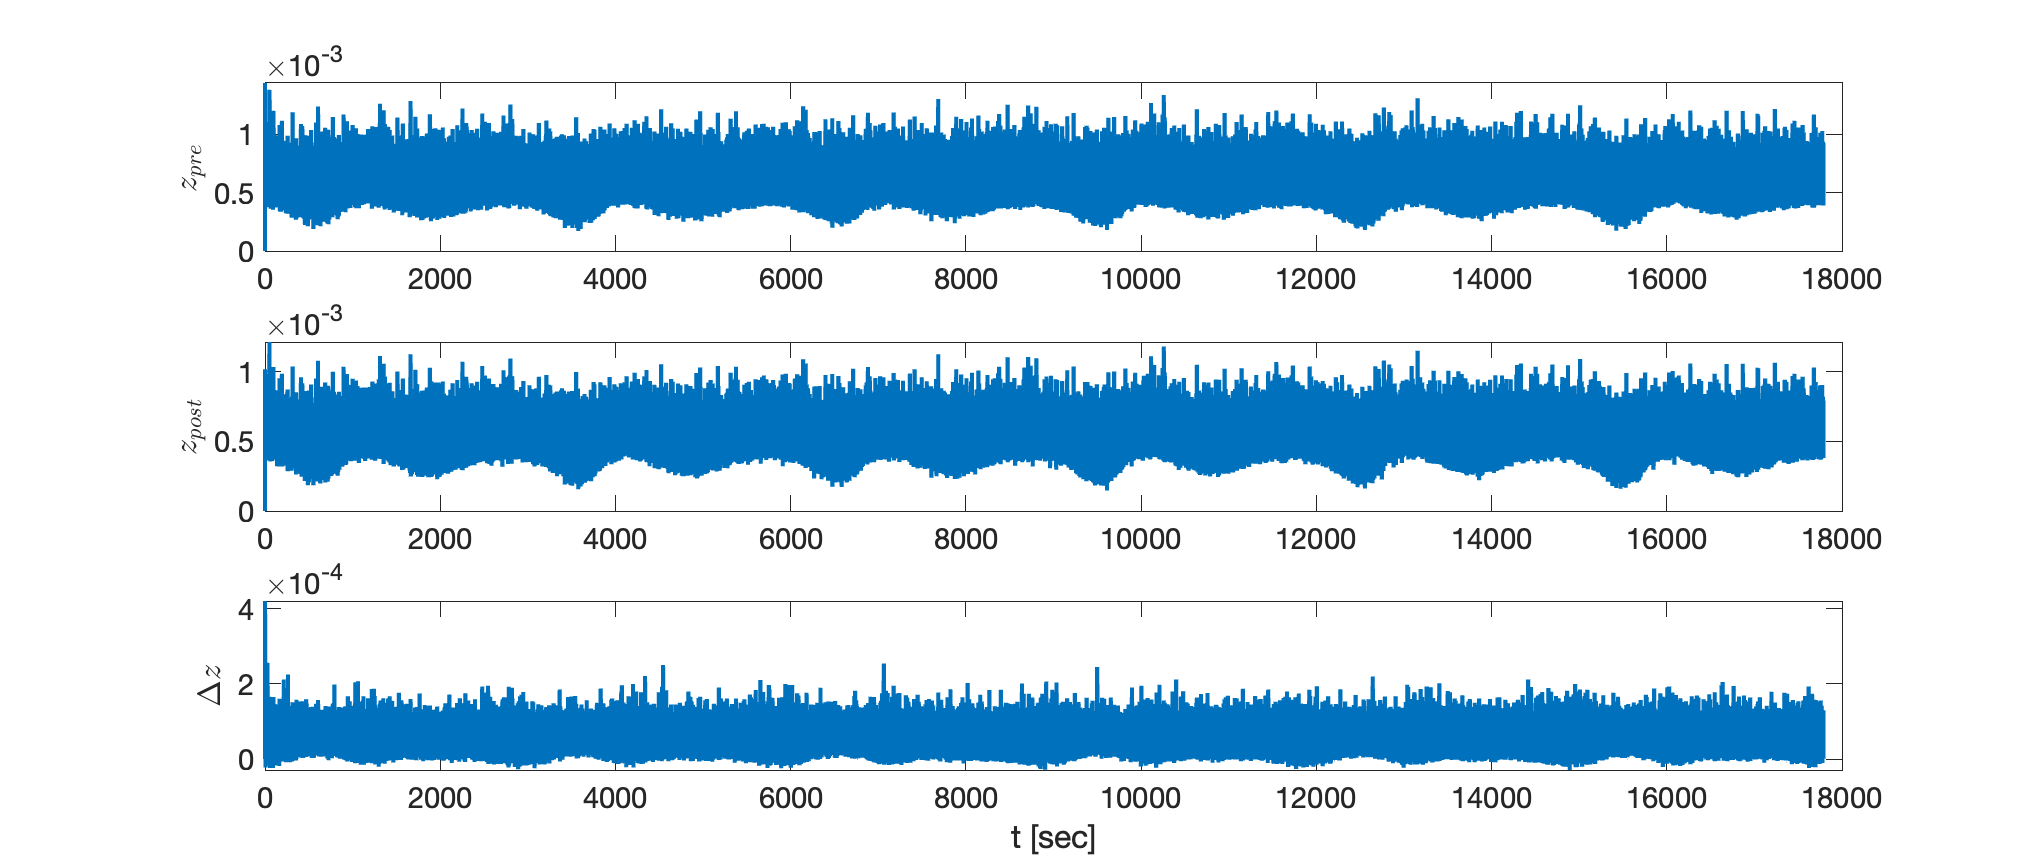
\includegraphics[width=12cm]{Images/PS10/mult_ext_kalman_filter_residual_comparison.png}
    \caption{Time History of Pre-fit Residual, Post-fit Residual, and Residual Difference}
    \label{fig:residual_norm_histories}
\end{figure}


% \subsection{Addition of Gyro Bias as State in MEKF}